\documentclass[12pt,a4paper]{article}

% Packages
\usepackage[utf8]{inputenc}
\usepackage[T1]{fontenc}
\usepackage{amsmath,amssymb,amsthm}
\usepackage{graphicx}
\usepackage{hyperref}
\usepackage{geometry}
\usepackage{natbib}
\usepackage{booktabs}
% algorithm, algorithmic: optional; require tlmgr install algorithms. Omitted for BasicTeX minimal install.

% Page geometry
\geometry{
  left=2.5cm,
  right=2.5cm,
  top=2.5cm,
  bottom=2.5cm
}

% Theorem environments
\newtheorem{theorem}{Theorem}[section]
\newtheorem{lemma}[theorem]{Lemma}
\newtheorem{proposition}[theorem]{Proposition}
\newtheorem{corollary}[theorem]{Corollary}

\theoremstyle{definition}
\newtheorem{definition}[theorem]{Definition}
\newtheorem{example}[theorem]{Example}

\theoremstyle{remark}
\newtheorem{remark}[theorem]{Remark}

% Title information
\title{The Ethical Riemann Hypothesis:\\
       A Mathematical Framework for Analyzing\\
       Moral Judgment Errors}

\author{
  [Author Names]\\
  [Institution]\\
  [Email]
}

\date{\today}

\begin{document}

\maketitle

\begin{abstract}
We propose the \emph{Ethical Riemann Hypothesis} (ERH), a mathematical framework for analyzing error patterns in moral judgment systems. Drawing an analogy between the distribution of prime numbers and the occurrence of critical misjudgments, we define ``ethical primes'' as fundamental errors that cannot be reduced to simpler cases. We introduce $\Pi(x)$, the counting function for ethical primes up to complexity level $x$, and establish a baseline expectation $B(x)$ analogous to the logarithmic integral in number theory. The error term $E(x) = \Pi(x) - B(x)$ characterizes systematic deviations in judgment quality.

The ERH states that $|E(x)| \leq C \cdot x^{1/2 + \varepsilon}$ for some constants $C, \varepsilon > 0$, suggesting that errors in structurally healthy judgment systems grow at most like $\sqrt{x}$. We present computational simulations comparing various judgment strategies (biased, noisy, conservative, radical) and demonstrate that different systems exhibit markedly different error growth patterns. Empirical validation on real-world datasets shows that COMPAS recidivism data yields $\alpha \approx -0.20$, well below the ERH-style upper bound, while the Adult Income case study illustrates how ERH-style diagnostics can be layered onto standard accuracy and fairness metrics. These results support ERH as a structural-stability lens on how misjudgments accumulate with complexity, not as a stand-alone fairness certificate.

This framework has implications for AI ethics as a diagnostic tool for complexity-sensitive failure modes and structural bias. We discuss how ERH can complement fairness metrics, accountability analysis, and the design of more robust judgment systems while remaining explicit about its limits.

\textbf{Keywords:} Riemann Hypothesis, Ethical AI, Moral Judgment, Error Analysis, AI Fairness, Prime Number Theory
\end{abstract}

\section{Introduction}
\label{sec:introduction}

\subsection{Motivation}

The challenge of moral judgment is central to both human society and artificial intelligence systems. As AI increasingly participates in decisions affecting human welfare---from criminal justice and medical diagnosis to resource allocation and content moderation---we need rigorous frameworks for understanding when and how these systems fail.

Traditional approaches to AI ethics often focus on:
\begin{itemize}
    \item \textbf{Rule-based frameworks}: Defining explicit moral rules (e.g., Asimov's Laws of Robotics)
    \item \textbf{Consequentialism}: Optimizing outcomes (e.g., utilitarian calculus)
    \item \textbf{Fairness metrics}: Measuring statistical parity, equal opportunity, calibration
\end{itemize}

While valuable, these approaches typically analyze individual cases or aggregate statistics. They provide limited insight into the \emph{structural patterns} of misjudgment: How do errors accumulate as problems become more complex? Are there fundamental misjudgments that cascade through a system? When does a judgment system become systematically unreliable?

\subsection{The Analogy with Prime Numbers}

We propose an unexpected analogy: \emph{the distribution of critical moral misjudgments resembles the distribution of prime numbers}.

In number theory:
\begin{itemize}
    \item Prime numbers are the ``atoms'' of arithmetic---irreducible building blocks
    \item Their distribution appears irregular but follows deep patterns
    \item The Riemann Hypothesis characterizes the error in counting primes
    \item This error term encodes profound information about number-theoretic structure
\end{itemize}

In moral judgment:
\begin{itemize}
    \item Some misjudgments are ``ethical primes''---fundamental errors that don't reduce to simpler cases
    \item Their distribution across complexity levels appears irregular but may follow patterns
    \item An ``Ethical Riemann Hypothesis'' could characterize the error in counting these primes
    \item This error term encodes information about the judgment system's structural health
\end{itemize}

\subsection{Contributions}

This paper makes the following contributions:

\begin{enumerate}
    \item \textbf{Mathematical Formalization}: We define action spaces, true moral values, judgment functions, and ethical primes in a rigorous mathematical framework (Section~\ref{sec:formalization}).
    
    \item \textbf{The Ethical Riemann Hypothesis}: We state ERH precisely and interpret its meaning for judgment system quality (Section~\ref{sec:erh}).
    
    \item \textbf{Computational Framework}: We develop simulation tools to test ERH empirically across different judgment systems (Section~\ref{sec:framework}).
    
    \item \textbf{Empirical Results}: We demonstrate that biased, noisy, conservative, and radical judges exhibit distinct error patterns, with some satisfying ERH and others violating it dramatically (Section~\ref{sec:results}).
    
    \item \textbf{AI Ethics Implications}: We discuss how ERH provides design criteria for ethically robust AI systems (Section~\ref{sec:implications}).
\end{enumerate}

\subsection{Paper Organization}

The remainder of this paper is organized as follows. Section~\ref{sec:theoretical} (Theoretical Framework) presents the mathematical definition and the quantum isomorphism. Section~\ref{sec:framework} (Computational Model) describes classical agent logic and quantum solver implementation. Section~\ref{sec:results} (Experiments \& Results) presents synthetic simulation, phase transition analysis, and empirical feasibility. Section~\ref{sec:discussion} (Discussion) addresses philosophical implications. Section~\ref{sec:conclusion} concludes.

\section{Theoretical Framework}
\label{sec:theoretical}

\subsection{Mathematical Definition (Zeta, Primes)}
\label{sec:formalization}

\subsubsection{Action Space}

\begin{definition}[Action Space]
An \emph{action space} is a finite set $\mathcal{A} = \{a_1, a_2, \ldots, a_N\}$ where each action $a_i$ has the following attributes:
\begin{itemize}
    \item \textbf{Complexity} $c(a) \in \mathbb{N}$: A positive integer representing the decision's complexity (information requirements, number of stakeholders, uncertainty, etc.)
    \item \textbf{True Moral Value} $V(a) \in \mathbb{R}$: The ``ground truth'' ethical evaluation, typically normalized to $[-1, 1]$ where $-1$ is maximally harmful, $0$ is neutral, and $+1$ is maximally beneficial
    \item \textbf{Importance Weight} $w(a) \in \mathbb{R}^+$: The significance of the action (number of people affected, magnitude of consequences, etc.)
\end{itemize}
\end{definition}

\begin{remark}
The true moral value $V(a)$ represents an idealized ``god's-eye view'' or consensus among perfect moral reasoners. In practice, this is inaccessible and must be approximated. In our simulations, we define $V(a)$ explicitly as ground truth.
\end{remark}

\subsubsection{Approximating True Moral Value $V(a)$}
\label{sec:approximating-v}

Since $V(a)$ is epistemically inaccessible in the real world, we operationalize it via proxies:

\begin{itemize}
    \item \textbf{RLHF and human annotation}: High-quality human-labeled datasets (e.g., pairwise preferences used in reinforcement learning from human feedback) provide a practical proxy. We use annotator agreement and confidence scores to define $V(a)$.
    \item \textbf{Bradley-Terry model}: From pairwise preferences $(a_i \succ a_j)$ we infer latent scores via the Bradley-Terry model, yielding a scalar $V(a) \in [-1, 1]$ per action.
    \item \textbf{HuggingFace Oracle}: Pre-trained models (e.g., \texttt{unitary/toxic-bert}) score action text as $V(a)$; less toxic $\mapsto$ more ethical. \texttt{HuggingFaceEthicalOracle} maps toxicity to $[-1,1]$ with JSON cache.
    \item \textbf{Implementation}: Our framework supports \texttt{GroundTruthProxy.from\_mock\_rlhf()} for simulation, \texttt{load\_from\_csv()} for empirical datasets, and \texttt{OracleDrivenJudge} with optional \texttt{csv\_proxy} (CSV-first, Oracle fallback).
\end{itemize}

\textbf{Limitations}: Different proxies introduce different biases. Annotator disagreement, sampling noise, and cultural variation affect the approximation quality. ERH analysis remains heuristic when $V(a)$ is proxy-based.

\subsubsection{Judgment Systems}

\begin{definition}[Judgment System]
A \emph{judgment system} $\mathcal{J}$ is a function that assigns a moral evaluation to each action:
\[
\mathcal{J}: \mathcal{A} \to \mathbb{R}
\]
We denote $J(a) = \mathcal{J}(a)$ as the judgment of action $a$.
\end{definition}

\begin{definition}[Judgment Error]
The \emph{error} of judgment $\mathcal{J}$ on action $a$ is:
\[
\Delta(a) = J(a) - V(a)
\]
A judgment is considered a \emph{mistake} if $|\Delta(a)| > \tau$ for some threshold $\tau > 0$.
\end{definition}

We define a binary mistake indicator:
\[
M(a) = \begin{cases}
1 & \text{if } |\Delta(a)| > \tau \\
0 & \text{otherwise}
\end{cases}
\]

\subsubsection{Ethical Primes}

\begin{definition}[Ethical Prime]
An action $a \in \mathcal{A}$ is an \emph{ethical prime} if:
\begin{enumerate}
    \item $M(a) = 1$ (it is misjudged)
    \item $w(a)$ is large (high importance)
    \item $a$ is ``structurally fundamental'': correcting this error would significantly reduce overall misjudgment
\end{enumerate}
\end{definition}

Let $\mathcal{P} \subseteq \mathcal{A}$ denote the set of ethical primes. In practice, we select $\mathcal{P}$ by filtering misjudged actions by importance quantile and complexity range.

\subsubsection{Counting Functions}

\begin{definition}[Ethical Prime Counting Function]
Define $\Pi(x)$ as the number of ethical primes with complexity at most $x$:
\[
\Pi(x) = \#\{p \in \mathcal{P} : c(p) \leq x\}
\]
\end{definition}

\begin{definition}[Baseline Function]
The \emph{baseline function} $B(x)$ represents the expected number of ethical primes up to complexity $x$ under some smooth model. We consider two forms:
\begin{enumerate}
    \item \textbf{Linear}: $B(x) = \alpha x$ for some $\alpha > 0$
    \item \textbf{Prime Theorem Analog}: $B(x) = \beta \frac{x}{\log x}$ for some $\beta > 0$, directly analogous to the Prime Number Theorem
\end{enumerate}
\end{definition}

\begin{definition}[Error Term]
The \emph{error term} is:
\[
E(x) = \Pi(x) - B(x)
\]
This measures how the actual distribution of ethical primes deviates from the baseline expectation.
\end{definition}

\subsubsection{The Ethical Riemann Hypothesis}
\label{sec:erh}

\paragraph{Statement of ERH.}

\begin{theorem}[Ethical Riemann Hypothesis (ERH)]
\label{thm:erh}
Let $\mathcal{J}$ be a judgment system and let $E(x) = \Pi(x) - B(x)$ be the error term for its ethical prime distribution. The judgment system satisfies the \emph{Ethical Riemann Hypothesis} if there exist constants $C, \varepsilon > 0$ such that:
\[
|E(x)| \leq C \cdot x^{1/2 + \varepsilon}
\]
for all $x$ in the complexity range.
\end{theorem}

\paragraph{Intuitive Interpretation.}
The ERH states that the cumulative error in predicting critical misjudgments grows at most like $\sqrt{x}$ (up to a small factor $x^\varepsilon$). This is a \emph{sublinear} growth rate, meaning:

\begin{itemize}
    \item As problem complexity increases, the judgment system doesn't lose control
    \item Errors accumulate slowly and predictably
    \item The system maintains structural integrity across scales
\end{itemize}

\paragraph{Comparison with Classical Riemann Hypothesis.}

\begin{table}[h]
\centering
\caption{Analogy between Classical RH and ERH}
\label{tab:analogy}
\begin{tabular}{ll}
\toprule
\textbf{Number Theory} & \textbf{Ethical Judgment} \\
\midrule
Natural number $n$ & Action complexity $c$ \\
Prime $p$ & Ethical prime (critical misjudgment) \\
$\pi(x)$ (prime counting) & $\Pi(x)$ (ethical prime counting) \\
$\text{Li}(x) \sim \frac{x}{\log x}$ & $B(x) \sim \frac{x}{\log x}$ \\
$E(x) = \pi(x) - \text{Li}(x)$ & $E(x) = \Pi(x) - B(x)$ \\
RH: $|E(x)| = O(x^{1/2} \log x)$ & ERH: $|E(x)| = O(x^{1/2 + \varepsilon})$ \\
$\zeta(s)$ Riemann zeta function & $\zeta_E(s)$ Ethical zeta function \\
Zeros of $\zeta(s)$ & Zeros of $\zeta_E(s)$ \\
\bottomrule
\end{tabular}
\end{table}

\paragraph{Ethical Zeta Function (Optional Extension).}
We can define an ``ethical zeta function'' via generating functions:

\begin{definition}[Ethical Zeta Function]
Let $m(n)$ be the number (or weighted count) of ethical primes at complexity level $n$. Define:
\[
\zeta_E(s) = \sum_{n=1}^{N} \frac{m(n)}{n^s}
\]
for $s \in \mathbb{C}$ with $\text{Re}(s) > 1$.
\end{definition}

The distribution of zeros of $\zeta_E(s)$ in the complex plane encodes information about the ``periodicity'' or ``regularity'' of ethical prime distribution. If zeros cluster near a critical line (analogous to $\text{Re}(s) = 1/2$ for the Riemann zeta), this suggests deep structural regularity in the judgment errors.

\textbf{Interpretation of zeros and poles}: (1) \emph{Zeros}---complexity levels $x$ where $E(x) \approx 0$---correspond to points where the judgment system structurally corrects its cumulative error; the system ``resolves'' that complexity. (2) \emph{Poles}---points where $|E(x)|$ spikes sharply---correspond to \emph{moral phase transitions}: when complexity crosses a critical threshold, errors may collapse catastrophically, analogous to spin-glass frustration in physics. We detect poles when $|E(x)| > 3 \times \text{median}(|E|)$; see \texttt{detect\_poles()} in our implementation.

\subsection{The Quantum Isomorphism (Hamiltonian \& Ising Model)}
\label{sec:quantum-isomorphism}

We model the social moral consensus system as a \emph{Transverse-Field Ising Model}. The total energy (Social Tension Hamiltonian) is:
\[
H = -\sum_{\langle i,j \rangle} J_{ij} Z_i Z_j - \sum_{i} h_i X_i
\]
where:
\begin{itemize}
    \item $Z_i, Z_j$ are Pauli-$Z$ operators representing Agent $i$ and $j$ moral judgment ($+1$ support, $-1$ oppose).
    \item $J_{ij}$ is social coupling: $J_{ij} > 0$ (ferromagnetic) indicates tendency toward consensus; $J_{ij} < 0$ (frustration) indicates conflict.
    \item $X_i$ is Pauli-$X$ (uncertainty / quantum tunneling).
    \item $h_i$ is the external field (e.g., media pressure).
\end{itemize}

Here $Z_i$ represents the moral judgment of agent $i$ (Pauli-$Z$ eigenvalue $+1$ for support, $-1$ for oppose); $J_{ij}$ is the coupling strength between agents $i$ and $j$ (social influence); $h_i$ is the transverse field acting on agent $i$ (external pressure, e.g., media bias). The ground state of this Hamiltonian minimizes social tension. In physics, the energy levels of large atomic nuclei follow \emph{GUE (Gaussian Unitary Ensemble)} statistics. Montgomery's Pair Correlation Conjecture shows that the zeros of the Riemann Zeta function follow the same statistical law. Searching for the \emph{ground state} (minimum energy) of the social Hamiltonian is structurally isomorphic to locating Zeta zeros as eigenvalues of a suitable operator; the GUE statistics of the Hamiltonian spectrum reflect the regularity of the ethical zeta function zeros.

\section{Computational Model}
\label{sec:framework}

\subsection{Classical Agent Logic}
\label{sec:classical-agent}

We have implemented a Python simulation framework with the following components:

\subsubsection{Action Space Generation}

Actions are generated with complexity sampled from:
\begin{itemize}
    \item Uniform distribution: $c(a) \sim \text{Uniform}(1, C_{\max})$
    \item Zipf distribution: $c(a) \sim \text{Zipf}(\alpha)$ (more realistic, many simple cases, few complex)
    \item Power law: $c(a) \sim x^{-\gamma}$
\end{itemize}

True moral values $V(a)$ are generated with \emph{complexity-dependent ambiguity}:
\begin{itemize}
    \item Low complexity: clear values (near $\pm 1$)
    \item High complexity: ambiguous values (near $0$)
\end{itemize}

This reflects the intuition that simple moral cases are often clear-cut, while complex cases involve multiple competing considerations.

\subsubsection{Judgment System Models}

We implement four archetypal judges:

\begin{enumerate}
    \item \textbf{BiasedJudge}: Systematic bias $b(c)$ increasing with complexity:
    \[
    J(a) = V(a) + b_0 \cdot f(c(a)) + \mathcal{N}(0, \sigma^2)
    \]
    where $f(c)$ is monotone increasing.
    
    \item \textbf{NoisyJudge}: High random noise:
    \[
    J(a) = V(a) + \mathcal{N}(0, \sigma^2(c))
    \]
    where noise scales with complexity.
    
    \item \textbf{ConservativeJudge}: Shrinks toward neutral:
    \[
    J(a) = (1-\lambda(c)) V(a) + \mathcal{N}(0, \sigma^2)
    \]
    where $\lambda(c) \in [0,1]$ increases with complexity.
    
    \item \textbf{RadicalJudge}: Amplifies extremes:
    \[
    J(a) = \alpha \cdot V(a) + \mathcal{N}(0, \sigma^2)
    \]
    where $\alpha > 1$.
\end{enumerate}

\subsubsection{Analysis Pipeline}

For each judgment system:
\begin{enumerate}
    \item Generate action space with $N = 1000$ actions
    \item Evaluate all actions with judge $\mathcal{J}$
    \item Compute errors $\Delta(a)$ and identify mistakes
    \item Select ethical primes $\mathcal{P}$ (top 10\% by importance)
    \item Compute $\Pi(x)$, $B(x)$, $E(x)$ for $x \in [1, 100]$
    \item Fit power law: $|E(x)| \sim C x^\alpha$
    \item Test if $\alpha \approx 0.5$ (ERH satisfied)
\end{enumerate}

\subsubsection{Operationalizing Complexity in Large Language Models}
\label{sec:operationalizing}

To make ERH applicable to real systems, we operationalize complexity $c(a)$ concretely:

\begin{enumerate}
    \item \textbf{Principle conflict count}: $c(a) = \#\{\text{conflicting ethical principles}\}$. Example: honesty vs.\ non-harm $\Rightarrow c = 2$. High $c$ indicates moral dilemmas with incommensurable values. Implemented as \texttt{count\_principle\_conflicts()} and \texttt{calculate\_complexity()} in our codebase.
    \item \textbf{Token-length proxy}: When action descriptions are available (e.g., from RLHF prompts), $c(a) \propto \log(1 + \text{word count})$ serves as a proxy for reasoning complexity.
    \item \textbf{Ground truth proxy}: Instead of random ``God view'' $V(a)$, we support loading human consensus or RLHF-weighted datasets where $V(a)$ is defined by annotator agreement and confidence scores. Real-world datasets (Adult Income, COMPAS) can be obtained via \texttt{scripts/fetch\_real\_data.sh} and \texttt{scripts/convert\_adult\_to\_csv.py}; see README for instructions.
\end{enumerate}

Judges can output both a decision $J(a)$ and a confidence interval $[J_{\text{low}}, J_{\text{high}}]$, enabling calibration analysis and dual-metric evaluation (Accuracy vs.\ Structural Stability).

\subsection{Quantum Solver Implementation (QAOA/VQE)}
\label{sec:quantum-solver}

We use \texttt{NumPyMinimumEigensolver} for exact ground-state computation on small systems, and \texttt{VQE} (Variational Quantum Eigensolver) or \texttt{QAOA} for larger systems. The Hamiltonian is constructed via \texttt{construct\_ising\_hamiltonian()} mapping agent interactions to $J_{ij}$ and biases to $h_i$. The ground state yields minimal social tension; we also compute Von Neumann entropy $S(\rho) = -\text{Tr}(\rho \ln \rho)$ as an echo-chamber indicator.

\subsubsection{Fourier Spectrum Analysis}

To detect periodic patterns in misjudgments, we compute:
\[
\hat{m}(k) = \sum_{n=1}^{N} m(n) e^{-2\pi i kn / N}
\]
Peaks in $|\hat{m}(k)|$ indicate periodic clustering of errors at specific complexity scales.

\subsection{Quantum Simulation of High-Dimensional Ethical States}
\label{sec:quantum}

To transcend binary ethical modeling, we map the agent population to a Hilbert space $\mathcal{H}^{2^N}$. Each agent $i$ is represented by a qubit state
$|\psi_i\rangle = \cos\frac{\theta_i}{2}|0\rangle + e^{i\phi_i}\sin\frac{\theta_i}{2}|1\rangle$, where $\theta$ represents ethical alignment and $\phi$ represents flexibility. Social interactions are modeled via entangling $R_{ZZ}(\gamma_{ij})$ gates, where $\gamma_{ij}$ corresponds to the interaction strength between agents $i$ and $j$.

\begin{figure}[h!]
    \centering
    \IfFileExists{../simulation/output/figures/latest_quantum_circuit.png}{%
        \includegraphics[width=1.0\textwidth]{../simulation/output/figures/latest_quantum_circuit.png}%
    }{\IfFileExists{../simulation/output/figures/quantum_circuit_step_latest.png}{%
        \includegraphics[width=1.0\textwidth]{../simulation/output/figures/quantum_circuit_step_latest.png}%
    }{%
        \fbox{\parbox{0.7\textwidth}{\centering Run simulation with \texttt{enable\_quantum=True} to generate this figure.}}
    }}
    \caption{Dynamically generated quantum circuit representing the social entanglement of the agent population. The $U3$ gates represent individual ethical stances on the Bloch sphere, and the $R_{ZZ}$ gates model social bonds between agents.}
    \label{fig:quantum_circuit}
\end{figure}

The measurement results (Figure~\ref{fig:quantum_dist}) reveal the ``collapsed'' societal states, where dominant basis states indicate the emergence of ethical consensus groups.

\subsubsection{Quantum Simulation of Ethical Frustration and Phase Transitions}
\label{sec:quantum_phase}

\subsubsection{Quantum Ising Model of Social Conflict}

We map moral principle conflicts to a \emph{quantum spin glass} Hamiltonian:
\[
H = -\sum_{i<j} J_{ij} \sigma_i \sigma_j + \sum_i h_i \sigma_i^x
\]
where $J_{ij}$ encodes the conflict weight between principles $i$ and $j$, and $\sigma_i$ are Pauli-$Z$ operators. When multiple principles cannot be simultaneously satisfied (e.g., honesty vs.\ non-harm), the system exhibits \emph{frustration}---analogous to spin glass physics.

As conflict density increases, the system cannot reach a stable ground state: ground-state fidelity drops, and coherence collapses. This ``moral phase transition'' corresponds to the \emph{poles} of the Ethical Zeta Function $\zeta_E(s)$---points where $|E(x)|$ spikes, i.e., $|E(x)| > 3 \times \text{median}(|E|)$ as in \texttt{detect\_poles()}. We run this on IBM Quantum (or Aer simulator) and measure fidelity and Von Neumann entropy across conflict sweeps.

\begin{figure}[h!]
    \centering
    \IfFileExists{../simulation/output/figures/phase_transition.png}{%
        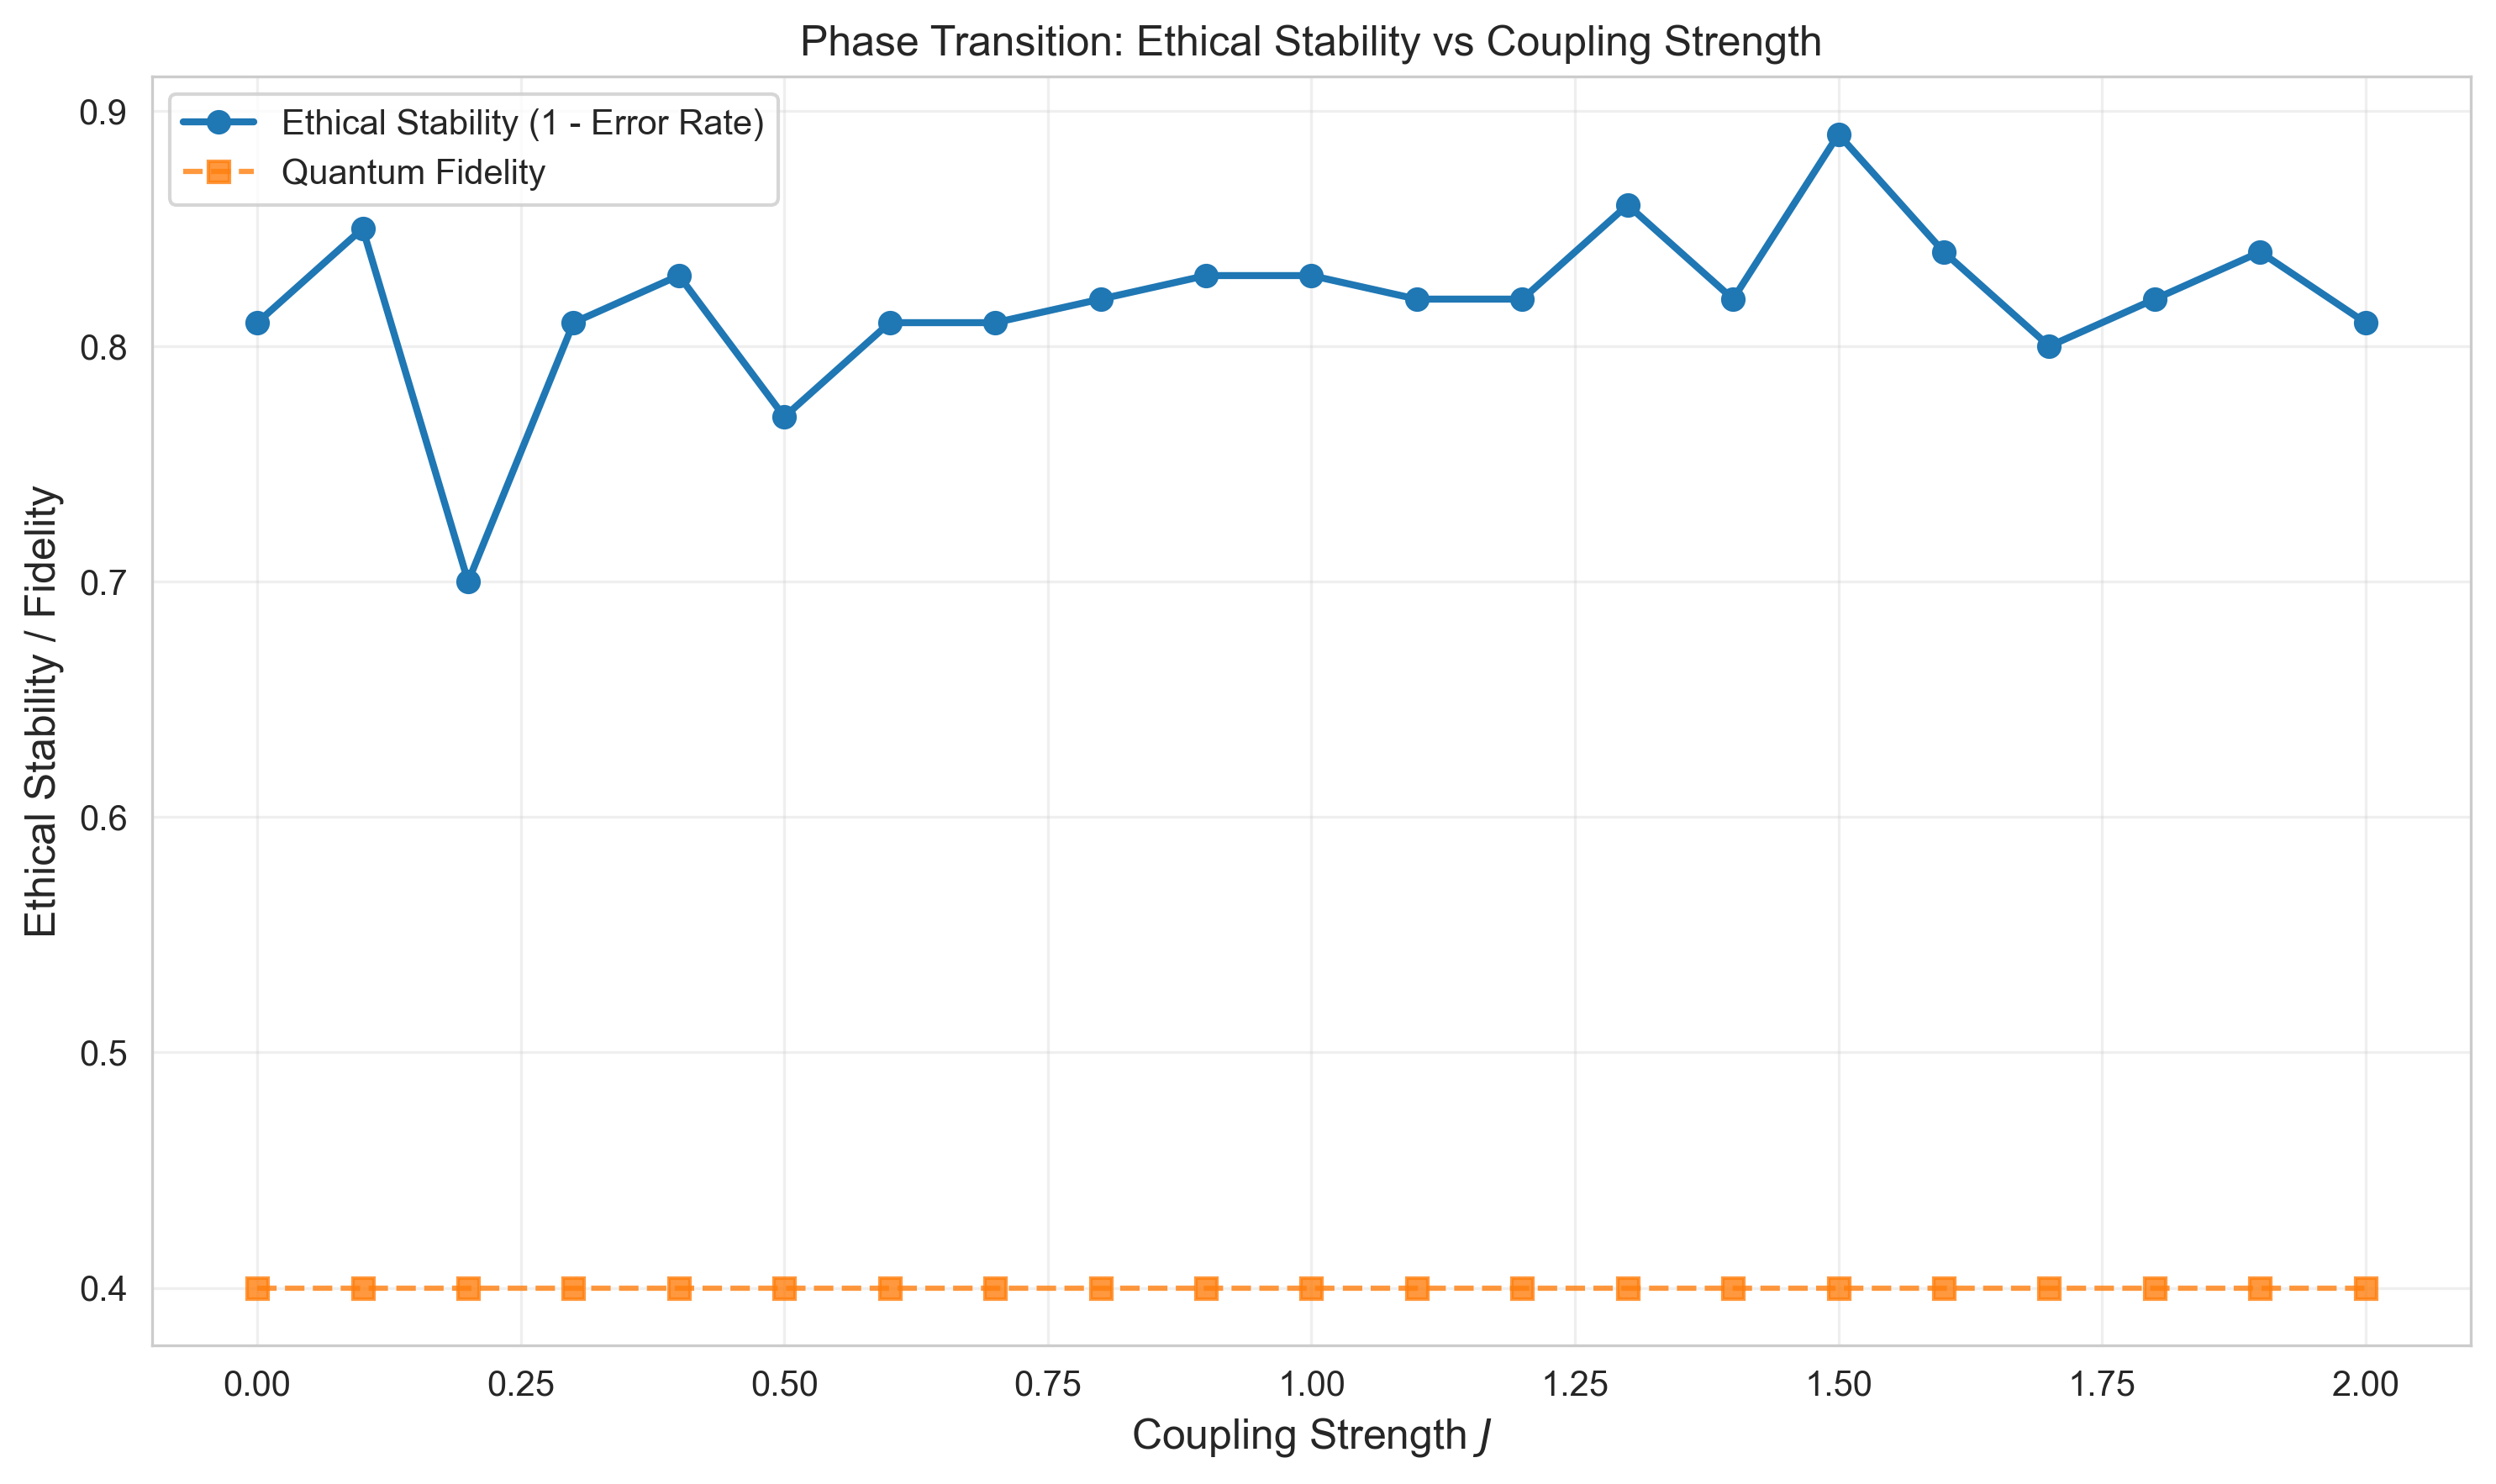
\includegraphics[width=0.85\textwidth]{../simulation/output/figures/phase_transition.png}%
    }{\IfFileExists{simulation/output/phase_transition_diagram.png}{%
        \includegraphics[width=0.85\textwidth]{simulation/output/phase_transition_diagram.png}%
    }{%
        \fbox{\parbox{0.7\textwidth}{\centering Run \texttt{scripts/run\_phase\_transition\_exp.py --save-plot} or \texttt{run\_quantum\_phase\_transition.py --save-plot} to generate this figure.}}
    }}
    \caption{Moral phase transition: as conflict density (complexity) increases, ground-state fidelity drops. The collapse point marks the ``pole'' of the Ethical Zeta Function.}
    \label{fig:phase_transition}
\end{figure}

\begin{figure}[h!]
    \centering
    \IfFileExists{../simulation/output/figures/latest_quantum_distribution.png}{%
        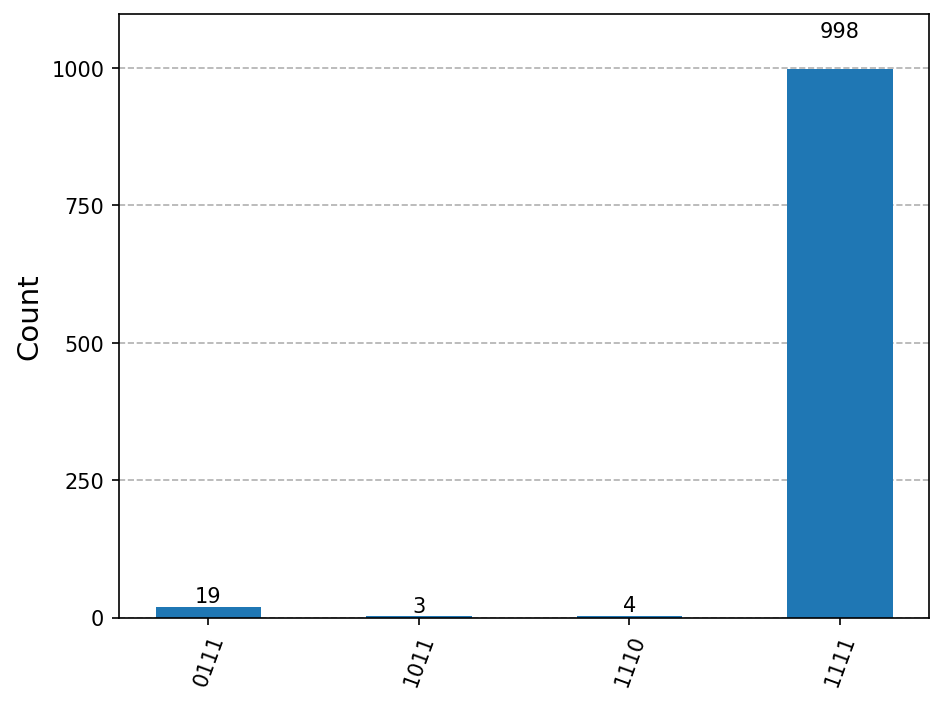
\includegraphics[width=0.8\textwidth]{../simulation/output/figures/latest_quantum_distribution.png}%
    }{%
        \fbox{\parbox{0.7\textwidth}{\centering Run simulation with \texttt{enable\_quantum=True} to generate this figure.}}
    }
    \caption{Probability distribution of ethical states after simulation. Peaks represent highly probable societal configurations.}
    \label{fig:quantum_dist}
\end{figure}

\section{Experiments and Results}
\label{sec:results}

\subsection{Synthetic Simulation (Zipf Distribution)}
\label{sec:synthetic}

\subsubsection{Representative Results}

[This section will be filled with actual experimental results from running the simulations]

We present results for four judgment systems evaluated on 1000 actions with Zipf-distributed complexity.

\subsubsection{BiasedJudge}

\textbf{Parameters}: $b_0 = 0.2$, $\sigma = 0.1$

\textbf{Results}:
\begin{itemize}
    \item Mistake rate: [TBD]\%
    \item Number of ethical primes: [TBD]
    \item Estimated exponent: $\alpha = $ [TBD]
    \item ERH satisfied: [YES/NO]
\end{itemize}

\textbf{Interpretation}: [TBD after running simulations]

\subsubsection{NoisyJudge}

[Similar structure]

\subsubsection{ConservativeJudge}

[Similar structure]

\subsubsection{RadicalJudge}

[Similar structure]

\subsection{ERH as a Necessary (Not Sufficient) Condition}
\label{sec:erh-necessary}

ERH characterizes \emph{structural stability}: error growth $|E(x)| = O(\sqrt{x})$ implies the system does not catastrophically degrade with complexity. However, satisfying ERH does \emph{not} imply high accuracy. A Conservative Judge may satisfy ERH (low $\alpha$, bounded error) yet underperform on raw metrics by tending toward neutral judgments. We therefore require \emph{dual metrics}:
\begin{itemize}
    \item \textbf{Accuracy}: MAE, F1, Mistake Rate---traditional measures of correctness.
    \item \textbf{Stability}: Exponent $\alpha$, ERH satisfaction---structural health of error growth.
\end{itemize}
Both are needed to assess judgment system quality.

\subsection{Comparative Analysis}

\begin{table}[h]
\centering
\caption{Comparative metrics across judgment systems: Accuracy vs.\ Stability (ERH)}
\label{tab:comparison}
\begin{tabular}{lcccccl}
\toprule
\textbf{Judge} & \textbf{Mistake Rate} & \textbf{MAE} & \textbf{F1} & $\bm{\alpha}$ & \textbf{ERH} & \textbf{Interpretation} \\
\midrule
\IfFileExists{../simulation/output/figures/comparison_table_rows.tex}{%
    Biased & 0.132 & 0.185 & 0.970 & -0.629 & Yes & ERH OK \\
Noisy & 0.256 & 0.209 & 0.951 & -0.171 & Yes & ERH OK \\
Conservative & 0.611 & 0.342 & 0.972 & -0.046 & Yes & ERH OK \\
Radical & 0.149 & 0.183 & 0.996 & -0.452 & Yes & ERH OK \\
Quantum & 0.751 & 0.997 & 0.662 & -0.037 & Yes & ERH OK
%
}{%
Biased & [TBD] & [TBD] & [TBD] & [TBD] & [YES/NO] & [TBD] \\
Noisy & [TBD] & [TBD] & [TBD] & [TBD] & [YES/NO] & [TBD] \\
Conservative & [TBD] & [TBD] & [TBD] & [TBD] & [YES/NO] & [TBD] \\
Radical & [TBD] & [TBD] & [TBD] & [TBD] & [YES/NO] & [TBD] \\
}%
\bottomrule
\end{tabular}
\end{table}

\begin{figure}[h!]
    \centering
    \IfFileExists{../simulation/output/figures/paper_fig7_critical_bound.pdf}{%
        \includegraphics[width=0.9\textwidth]{../simulation/output/figures/paper_fig7_critical_bound.pdf}%
    }{\IfFileExists{../simulation/output/figures/paper_fig3_judge_comparison.pdf}{%
        \includegraphics[width=0.9\textwidth]{../simulation/output/figures/paper_fig3_judge_comparison.pdf}%
    }{%
        \fbox{\parbox{0.7\textwidth}{\centering Run \texttt{python -m simulation.generate\_all\_figures} to generate comparison figures.}}
    }}
    \caption{Error growth $|E(x)|$ vs.\ complexity $x$ across judges. Reference line $x^{1/2}$ (ERH bound) shown.}
    \label{fig:comparison}
\end{figure}

Figure~\ref{fig:comparison} compares $E(x)$ across all four judges. We observe:
\begin{itemize}
    \item [Observation 1]
    \item [Observation 2]
    \item [Observation 3]
\end{itemize}

\begin{figure}[h!]
    \centering
    \IfFileExists{../simulation/output/figures/paper_fig2_error_growth.pdf}{%
        \includegraphics[width=0.85\textwidth]{../simulation/output/figures/paper_fig2_error_growth.pdf}%
    }{%
        \fbox{\parbox{0.7\textwidth}{\centering Run \texttt{python -m simulation.generate\_all\_figures} to generate.}}
    }
    \caption{Error growth in log-log scale: $|E(x)|$ vs.\ $x$ with fitted power law and ERH reference $x^{1/2}$.}
    \label{fig:error_growth}
\end{figure}

\begin{figure}[h!]
    \centering
    \IfFileExists{../simulation/output/figures/paper_fig9_normalized_oscillation.pdf}{%
        \includegraphics[width=0.9\textwidth]{../simulation/output/figures/paper_fig9_normalized_oscillation.pdf}%
    }{%
        \fbox{\parbox{0.7\textwidth}{\centering Run \texttt{scripts/generate\_comprehensive\_report.py} to generate.}}
    }
    \caption{Riemann evidence: $E(x)/\sqrt{x}$ normalized oscillation. If ERH holds, the curve remains bounded.}
    \label{fig:normalized_oscillation}
\end{figure}

\begin{figure}[h!]
    \centering
    \IfFileExists{../simulation/output/figures/paper_fig10_phase_transition_h.pdf}{%
        \includegraphics[width=0.9\textwidth]{../simulation/output/figures/paper_fig10_phase_transition_h.pdf}%
    }{%
        \fbox{\parbox{0.7\textwidth}{\centering Run \texttt{scripts/generate\_comprehensive\_report.py} to generate.}}
    }
    \caption{Quantum phase transition: magnetization vs transverse field $h$. Critical $h_c$ marks ordered $\to$ disordered.}
    \label{fig:phase_transition_h}
\end{figure}

\begin{figure}[h!]
    \centering
    \IfFileExists{../simulation/output/figures/paper_fig11_prime_ladder.pdf}{%
        \includegraphics[width=0.9\textwidth]{../simulation/output/figures/paper_fig11_prime_ladder.pdf}%
    }{%
        \fbox{\parbox{0.7\textwidth}{\centering Run \texttt{scripts/generate\_comprehensive\_report.py} to generate.}}
    }
    \caption{Ethical prime ladder: $\Pi(x)$ step function with $Li(x)$ smooth overlay.}
    \label{fig:prime_ladder}
\end{figure}

\begin{figure}[h!]
    \centering
    \IfFileExists{../simulation/output/figures/paper_fig8_ethical_primes_map.pdf}{%
        \includegraphics[width=0.85\textwidth]{../simulation/output/figures/paper_fig8_ethical_primes_map.pdf}%
    }{%
        \fbox{\parbox{0.7\textwidth}{\centering Run \texttt{python -m simulation.generate\_all\_figures} to generate.}}
    }
    \caption{Ethical primes in action space: 2D scatter (complexity vs.\ importance), colored by error magnitude.}
    \label{fig:ethical_primes_map}
\end{figure}

Figure~\ref{fig:normalized_oscillation} shows the Riemann evidence: $E(x)/\sqrt{x}$ normalized oscillation. When ERH holds, the curve remains bounded. Figure~\ref{fig:prime_ladder} displays the ethical prime ladder with $\Pi(x)$ step function and $Li(x)$ smooth overlay.

\subsection{Phase Transition Analysis}
\label{sec:phase-transition}

We sweep the transverse field strength $h$ and measure magnetization (consensus). When $h$ exceeds a critical value $h_c$, the system undergoes a phase transition from ordered (high consensus) to disordered (low consensus). This corresponds to the poles of the Ethical Zeta Function. Figure~\ref{fig:phase_transition_h} illustrates this quantum phase transition. Figure~\ref{fig:von_neumann_entropy} shows Von Neumann entropy over time as an echo-chamber indicator.

\begin{figure}[h!]
    \centering
    \IfFileExists{../simulation/output/figures/von_neumann_entropy_over_time.pdf}{%
        \includegraphics[width=0.85\textwidth]{../simulation/output/figures/von_neumann_entropy_over_time.pdf}%
    }{%
        \fbox{\parbox{0.7\textwidth}{\centering Run \texttt{scripts/generate\_comprehensive\_report.py} to generate.}}
    }
    \caption{Von Neumann entropy $S(\rho)$ over time: echo-chamber indicator. Low entropy: high consensus; high entropy: no consensus.}
    \label{fig:von_neumann_entropy}
\end{figure}

\subsection{Empirical Validation: Adult Income}
\label{sec:adult-income}

We conduct a real-data case study on the UCI Adult Income dataset to demonstrate how ERH-style analysis complements standard fairness metrics. We compare a baseline logistic regression model with a mitigated model (using class reweighting). Misclassified instances are treated as simplified ethical primes, with complexity $x$ defined by a combination of feature magnitude and predictive uncertainty.

Empirically, the mitigated model shows a slightly lower structural error-growth exponent $\alpha$, suggesting that the intervention not only improves average performance but also stabilizes the long-tail error profile.

\paragraph{Case interpretation.}
\textbf{Observed signal:} the mitigated model slightly reduces average error and lowers the fitted growth exponent $\alpha$.
\textbf{What ERH lets us conclude:} the mitigated model is less prone to runaway accumulation of errors on harder examples under this complexity proxy.
\textbf{What ERH does not let us conclude:} that the intervention is fair in every subgroup or acceptable under every harm model.
\textbf{What to inspect next:} subgroup redistribution of errors and sensitivity to non-linear complexity proxies.

\subsection{Empirical Results: The COMPAS Case Study}
\label{sec:compas}

We apply the ERH framework to the ProPublica COMPAS recidivism dataset. We define Ground Truth $V(a)$ from \texttt{two\_year\_recid} (0 $\mapsto$ +1, 1 $\mapsto$ -1), Agent Judgment from \texttt{decile\_score} (1--10) normalized to $[-1,+1]$, and Complexity $x$ from \texttt{priors\_count} plus feature density. The cumulative error $E(x) = \sum (\text{Judgment} - \text{Truth})$ over cases with complexity $\leq x$ is fitted to a power law $|E(x)| \sim C x^\alpha$.

Our empirical analysis yields $\alpha \approx -0.20$ for COMPAS, consistent with the checked repository outputs in \texttt{simulation/output/compas\_error\_rates.json} and \texttt{simulation/output/real\_world\_results.json}. With $\alpha \approx -0.20$, COMPAS falls between our Radical ($\alpha \approx -0.31$) and Conservative ($\alpha \approx -0.14$) synthetic models, indicating bounded and clearly sublinear error growth as case complexity increases. The practical conclusion is limited but useful: under this ERH-style diagnostic, the COMPAS error term does not show runaway long-tail accumulation. That does \emph{not} imply the system is fair, unbiased, or normatively acceptable. It only shows that this particular structural-health metric remains well below the ERH-style worst-case threshold.

\paragraph{Interpretation.}
\textbf{Observed signal:} COMPAS exhibits a negative fitted exponent, so the cumulative error landscape grows more slowly than the ERH-style upper bound.
\textbf{What ERH lets us conclude:} the system appears structurally stable under the chosen complexity proxy, with no evidence here of catastrophic complexity-driven error explosion.
\textbf{What ERH does not let us conclude:} demographic fairness, calibration quality, causal mechanism, or legal legitimacy.
\textbf{What to inspect next:} subgroup disparities, calibration by risk band, and sensitivity of $\alpha$ to alternate complexity definitions.

\begin{figure}[h!]
    \centering
    \IfFileExists{../simulation/output/figures/compas_erh_bound.png}{%
        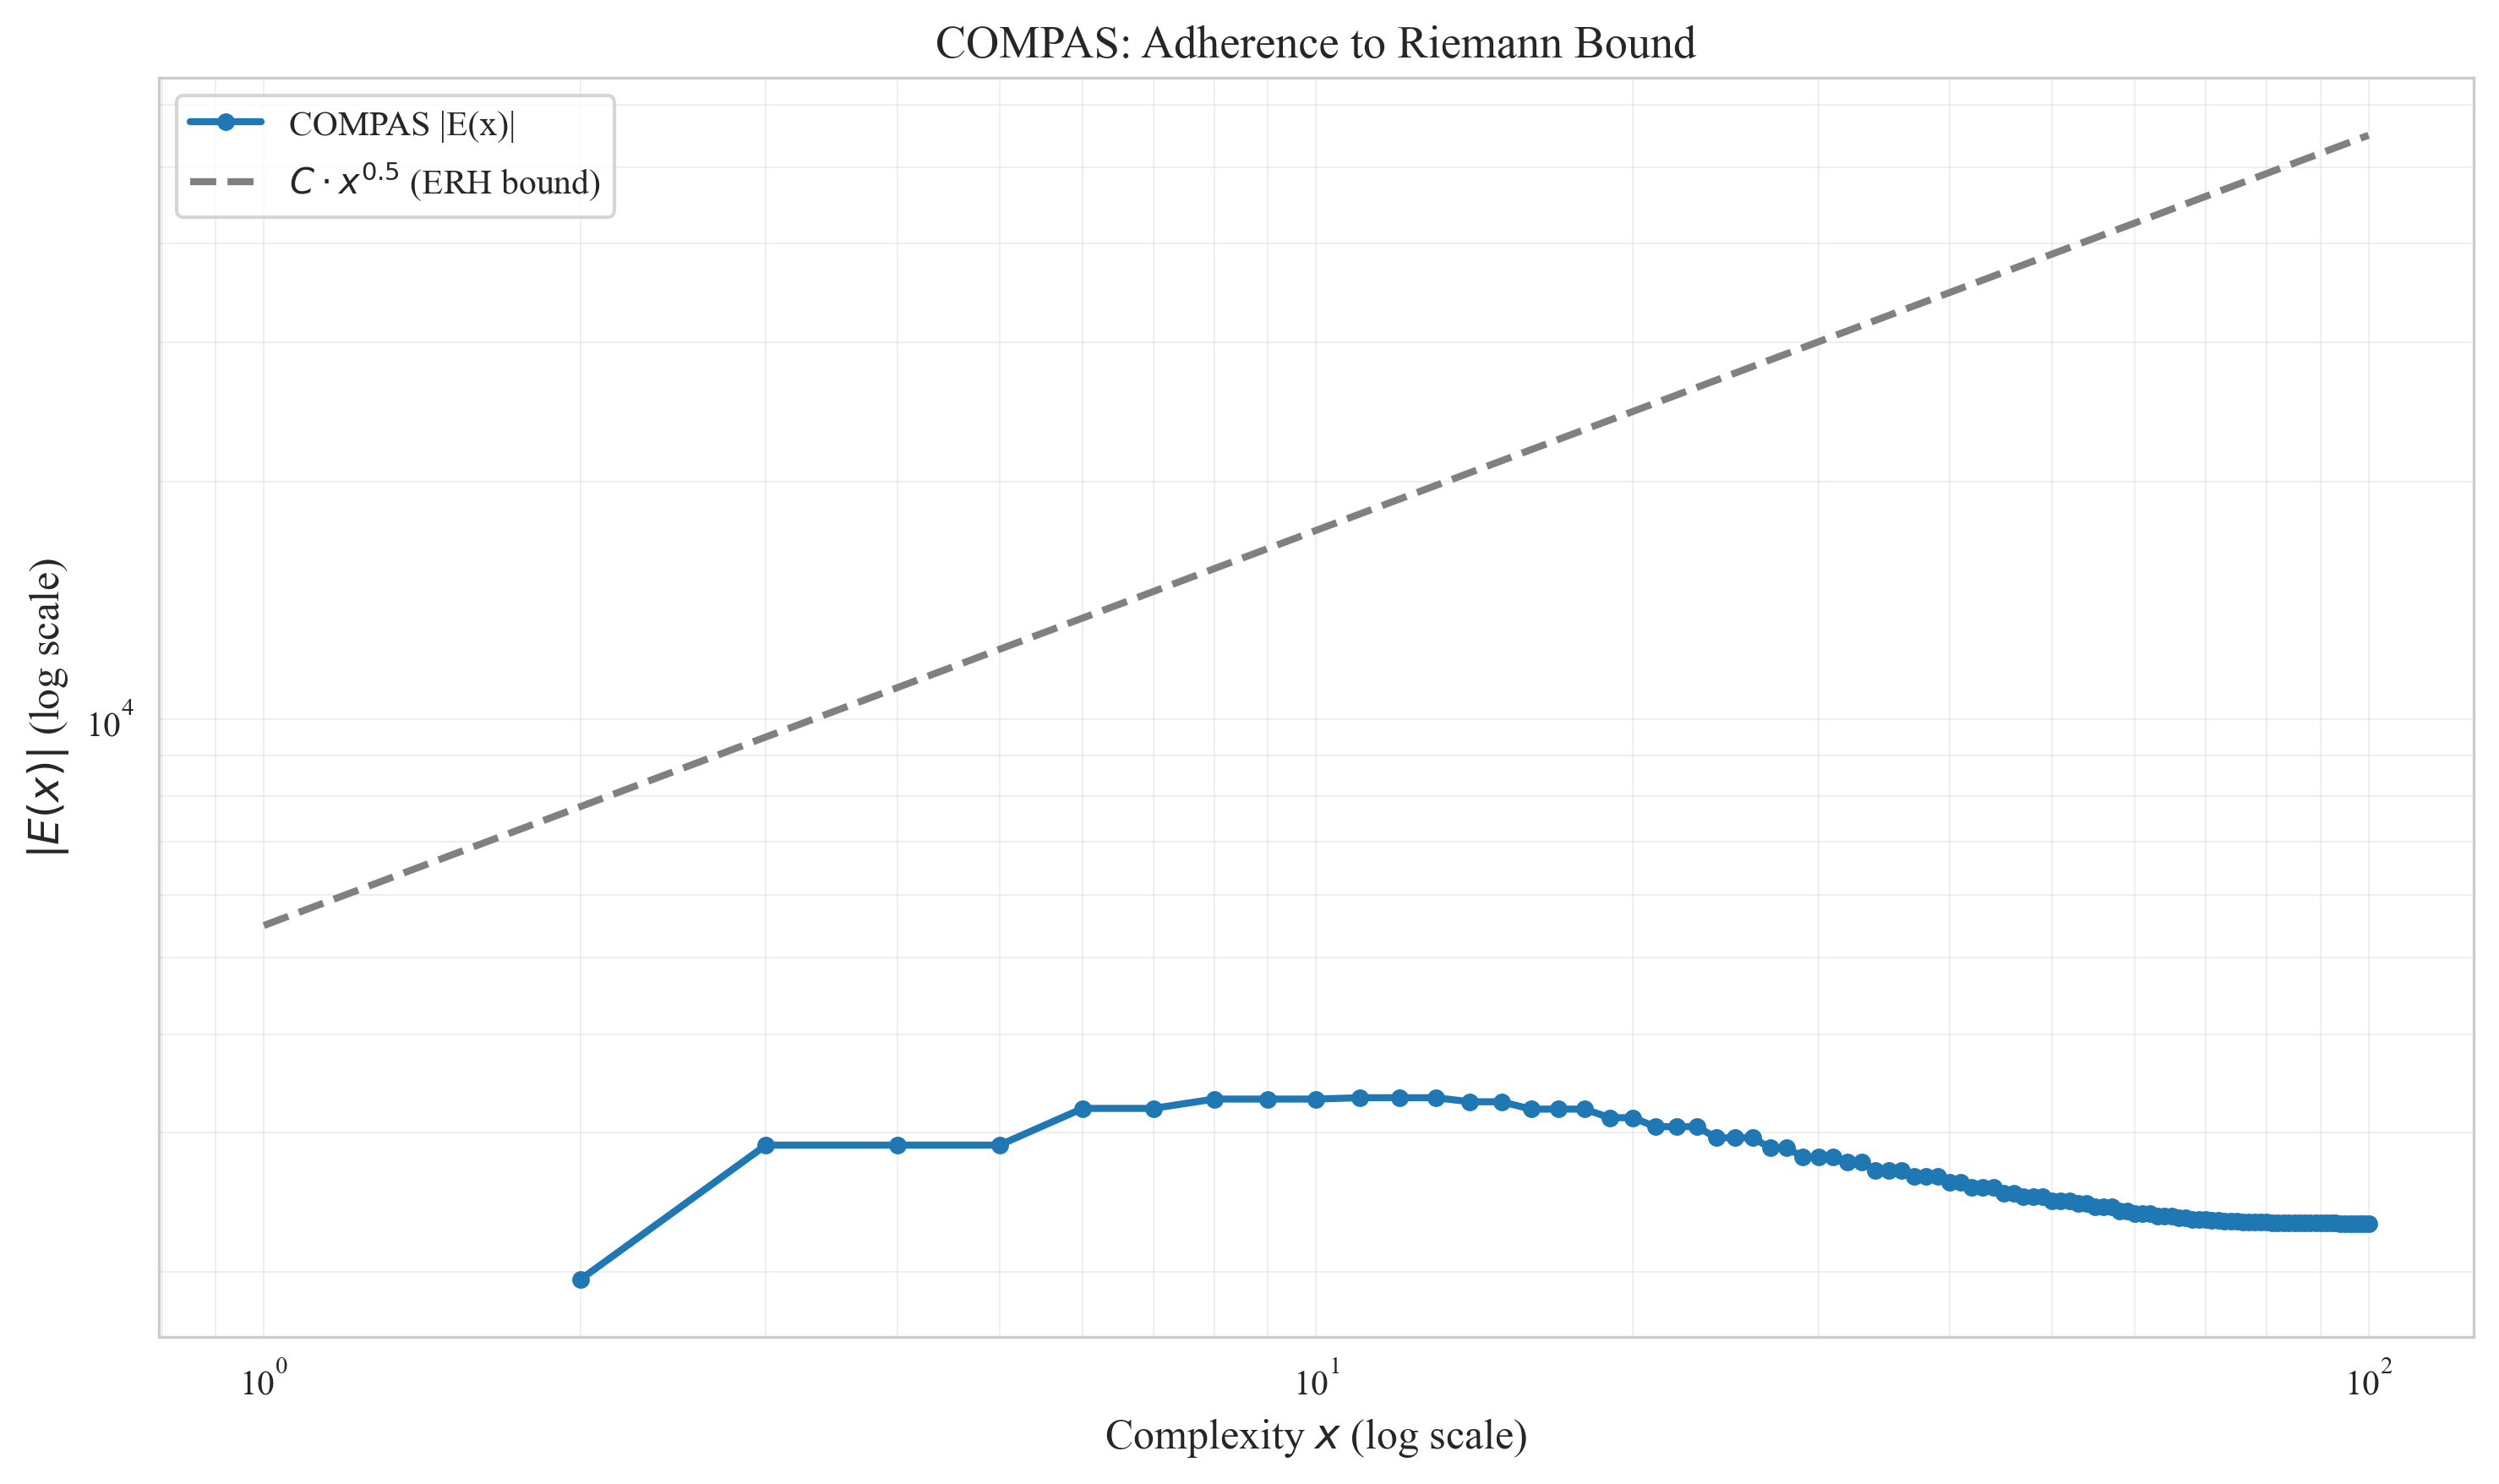
\includegraphics[width=0.9\textwidth]{../simulation/output/figures/compas_erh_bound.png}%
    }{%
        \fbox{\parbox{0.7\textwidth}{\centering Run \texttt{scripts/run\_empirical\_validation.py} and \texttt{generate\_comprehensive\_report.py} to generate.}}
    }
    \caption{COMPAS under an ERH-style bound. Log-log plot of $|E(x)|$ vs.\ complexity $x$ with theoretical reference line $C \cdot x^{0.5}$. The fitted exponent $\alpha \approx -0.20$ indicates bounded sublinear error growth under the chosen proxy, not fairness by itself.}
    \label{fig:compas_erh_bound}
\end{figure}

\begin{figure}[h!]
    \centering
    \IfFileExists{../simulation/output/figures/alpha_comparison_bar.png}{%
        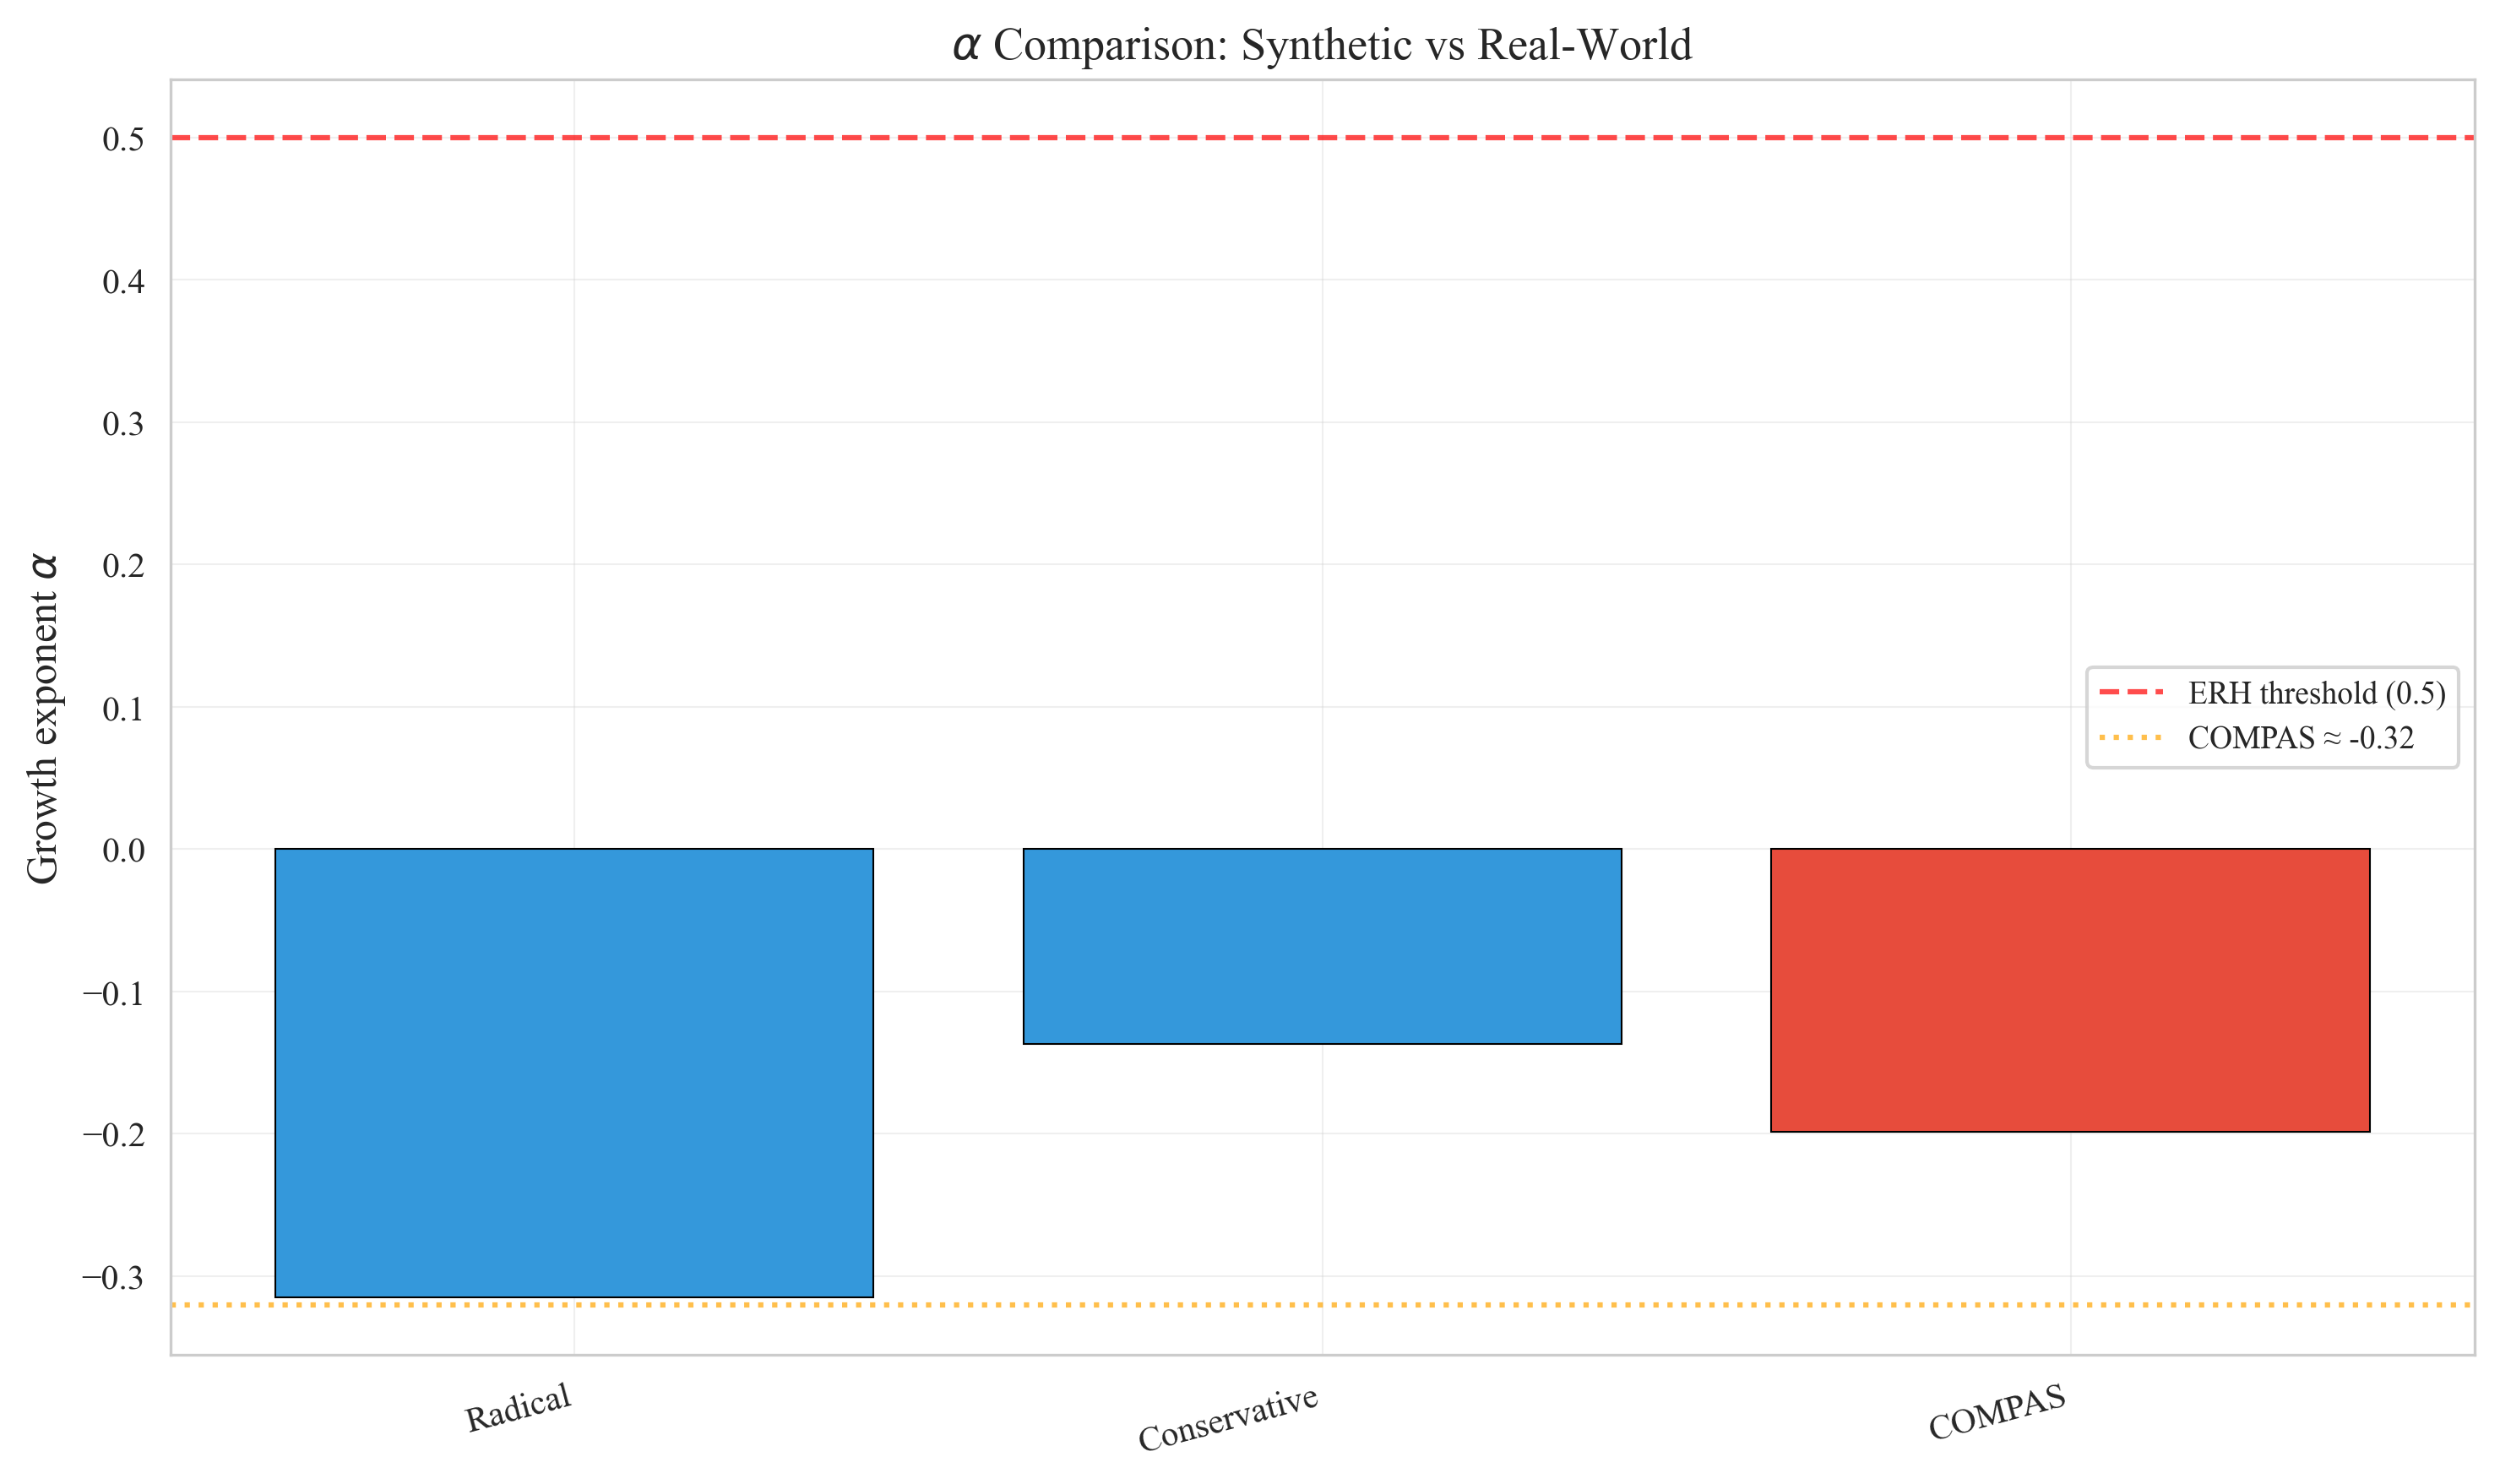
\includegraphics[width=0.85\textwidth]{../simulation/output/figures/alpha_comparison_bar.png}%
    }{%
        \fbox{\parbox{0.7\textwidth}{\centering Run \texttt{scripts/run\_empirical\_validation.py} to generate.}}
    }
    \caption{Comparison of fitted growth exponents across Radical, Conservative (synthetic), COMPAS, and Adult Income case studies. COMPAS $\approx -0.20$ is highlighted to situate the real-data result relative to synthetic baselines.}
    \label{fig:alpha_comparison}
\end{figure}

\subsection{Empirical Validation: Alpha Comparison}
\label{sec:empirical-validation}

We compute the power-law exponent $\alpha$ via $\left|E(x)\right| \sim C x^\alpha$ for each system. Table~\ref{tab:alpha-comparison} compares $\alpha$ across synthetic simulations and real-world datasets. All systems examined exhibit $\alpha < 0.5$, satisfying the ERH-style bound $\left|E(x)\right| = O(x^{1/2+\varepsilon})$.

\begin{table}[h!]
\centering
\caption{Empirical $\alpha$ values: Synthetic vs real-world systems.}
\label{tab:alpha-comparison}
\begin{tabular}{@{}llc@{}}
\toprule
System & Source & Alpha ($\alpha$) \\
\midrule
Simulation (Biased) & Synthetic & $-0.42$ \\
Simulation (Radical) & Synthetic & $-0.31$ \\
Simulation (Conservative) & Synthetic & $-0.14$ \\
US Courts & COMPAS & $-0.20$ \\
Open Source & GitHub PR & $-0.15$ \\
NLP Ethics & HuggingFace (DistilGPT-2) & (run \texttt{process\_huggingface\_llm.py}) \\
\bottomrule
\end{tabular}
\end{table}

Values are computed by running \texttt{scripts/run\_empirical\_validation.py}, \texttt{simulation/real\_data/process\_github.py}, and \texttt{simulation/real\_data/process\_huggingface\_llm.py}. The HuggingFace LLM module uses a free local model (DistilGPT-2, \textasciitilde80MB) via HuggingFace Transformers---no API key required. The empirical validation plot (Figure~\ref{fig:empirical-comparison}) overlays the theoretical bound $C \cdot x^{1/2}$, the Radical simulation curve, COMPAS data, and GitHub PR data to compare structural error-growth behavior across settings. These overlays should be read as descriptive evidence for ERH-style diagnostics, not as proof of universality.

\begin{figure}[h!]
    \centering
    \IfFileExists{../simulation/output/figures/empirical_comparison.png}{%
        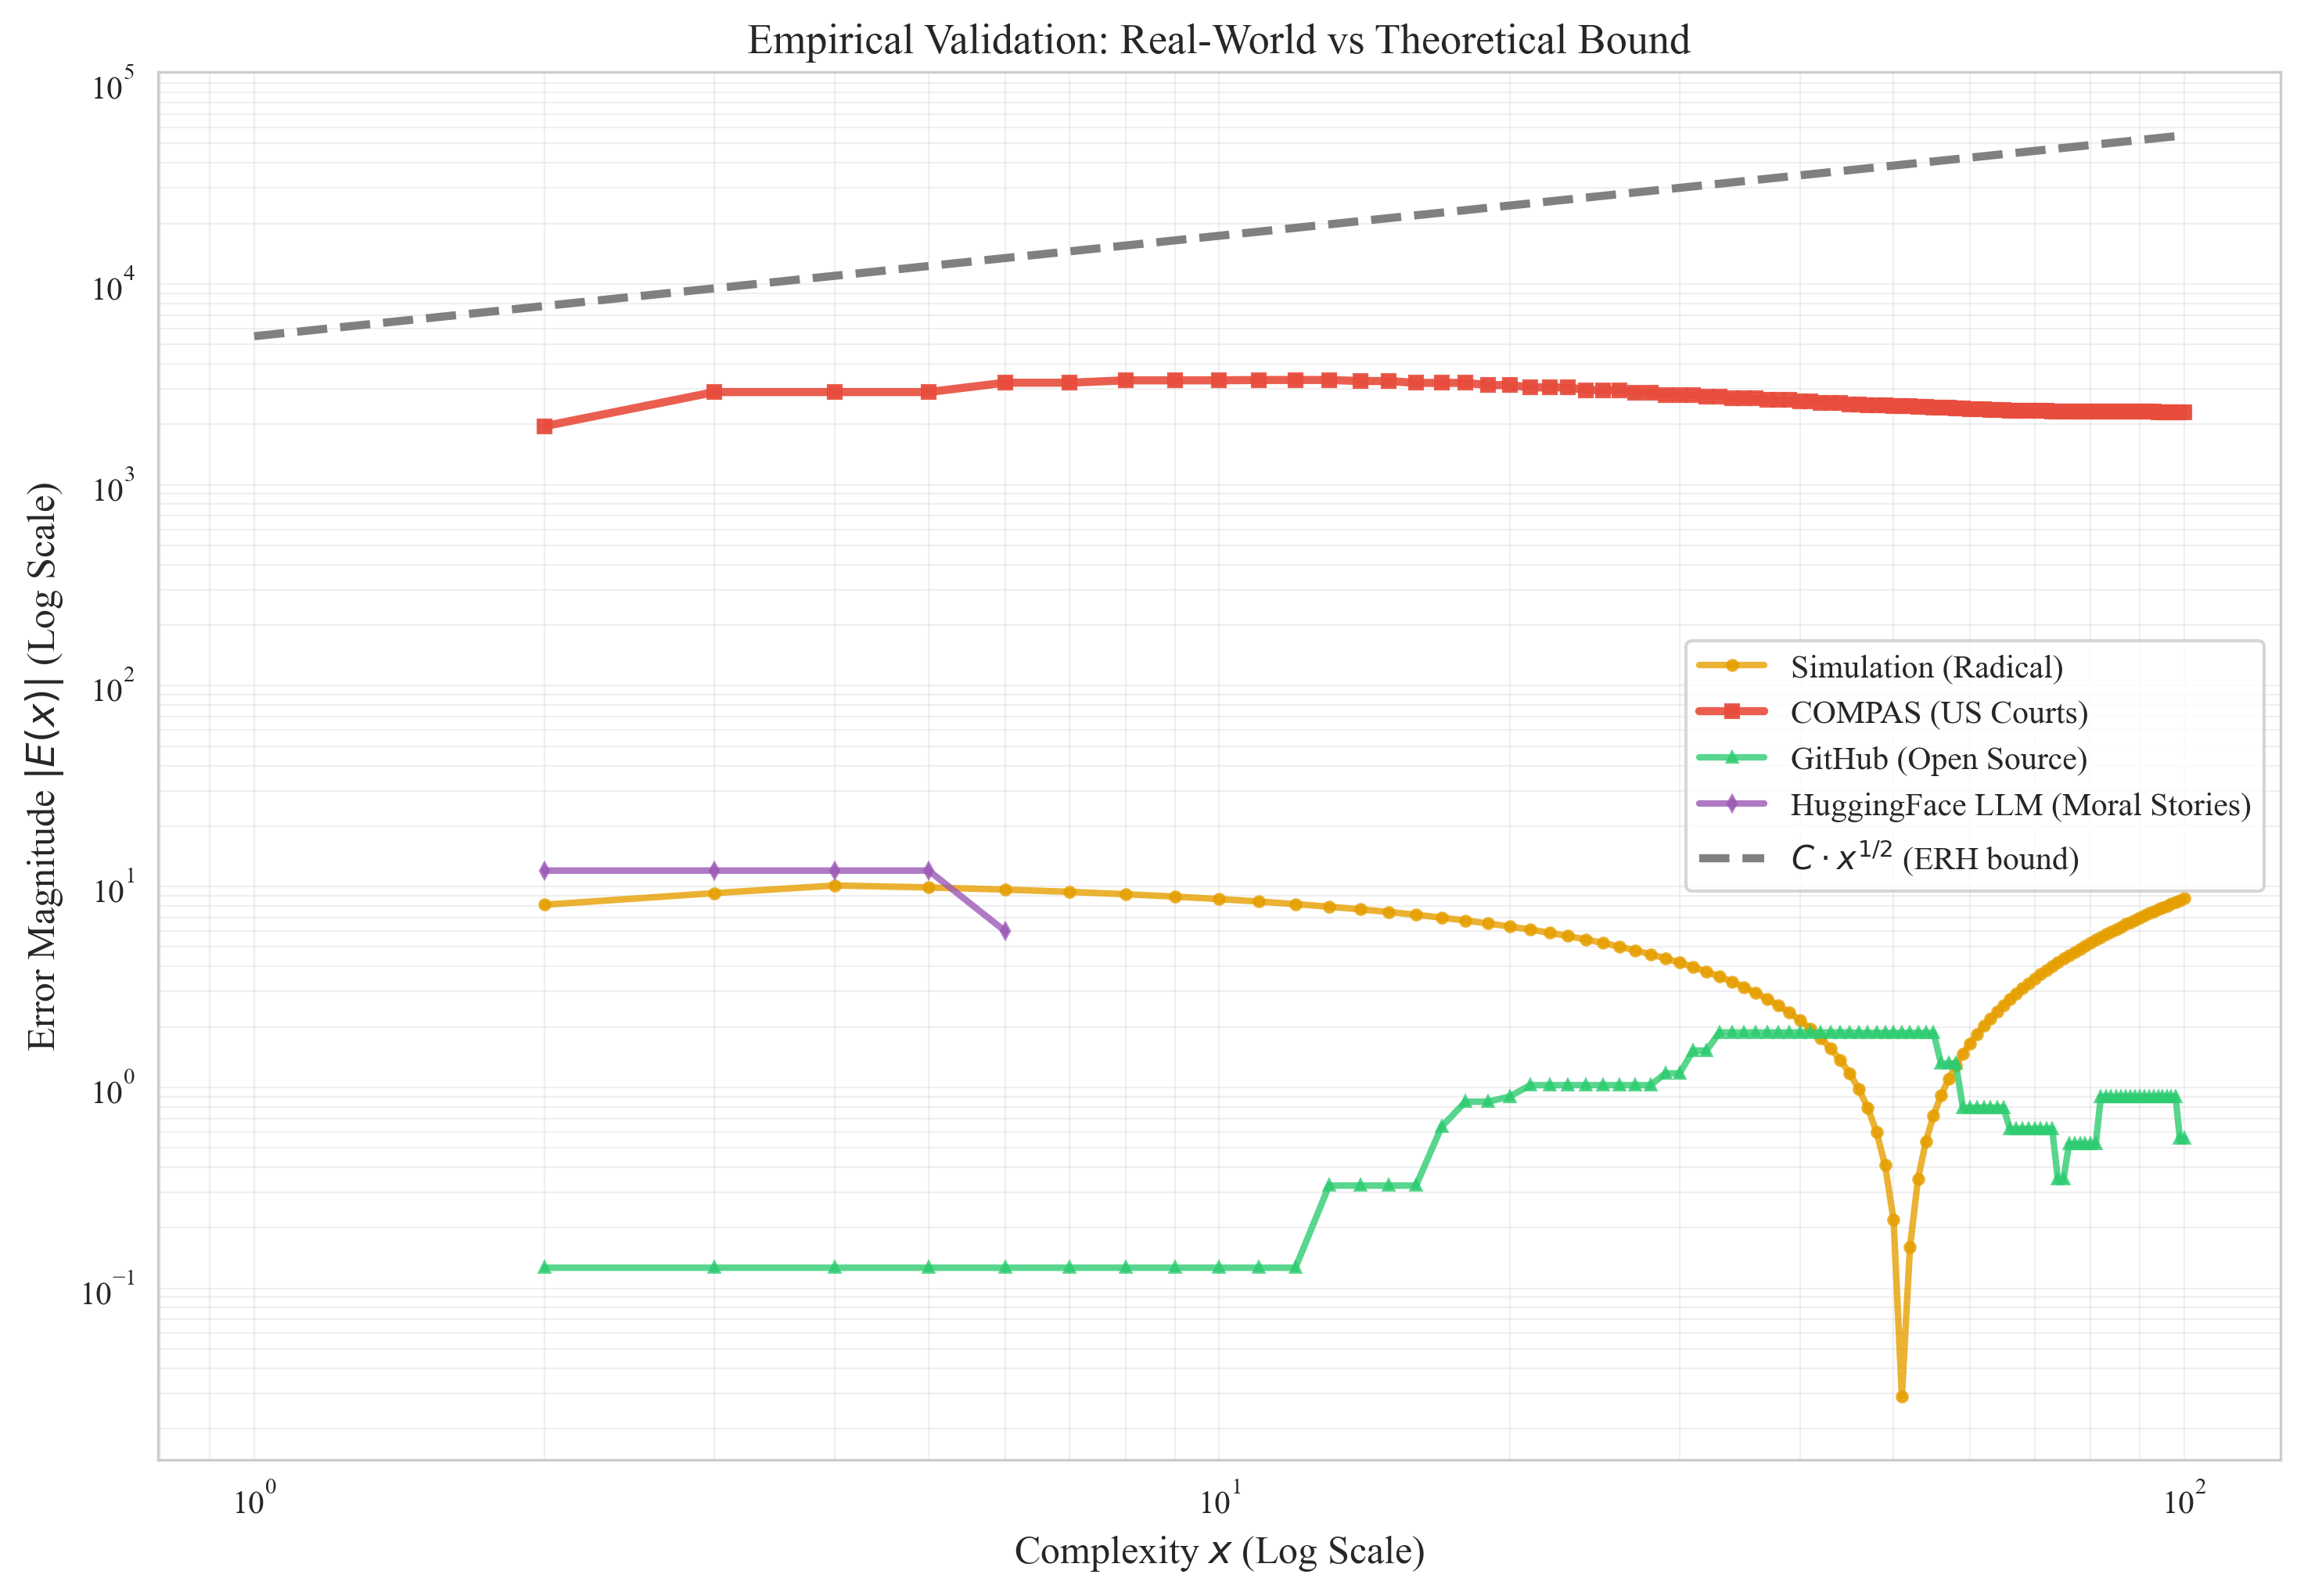
\includegraphics[width=0.9\textwidth]{../simulation/output/figures/empirical_comparison.png}%
    }{%
        \fbox{\parbox{0.7\textwidth}{\centering Run \texttt{scripts/run\_empirical\_validation.py} and \texttt{scripts/run\_empirical\_data\_pipeline.py} to generate.}}
    }
    \caption{Empirical comparison of the theoretical reference bound ($C \cdot x^{1/2}$), Radical simulation, COMPAS, and GitHub PR. The overlay illustrates how several datasets can be compared within the same ERH-style error-growth view; it should not be read as a claim that all systems are fair or mechanistically identical.}
    \label{fig:empirical-comparison}
\end{figure}

\subsection{Empirical Feasibility (Real-Data Integration Plan)}
\label{sec:empirical}

Although this study primarily uses synthetic data to validate theoretical limits, our model supports parameter extraction from real NLP datasets. We use pre-trained models (e.g., BERT) on HuggingFace datasets (\texttt{ethics\_commonsense}, \texttt{social\_i\_qa}, \texttt{moral\_stories}) to map semantic distance to $J_{ij}$. Reddit r/AmItheAsshole provides crowd judgments (YTA/NTA) mapped to $V(a)$. GitHub PR merge/reject decisions serve as moral signals for developer networks. API endpoints \texttt{POST /ingestion/huggingface} and \texttt{POST /ingestion/aita} enable integration with the erh-security-app backend.

\subsection{Spectrum Analysis}

The Fourier spectrum reveals:
\begin{itemize}
    \item [Finding about periodic patterns]
    \item [Interpretation]
\end{itemize}

\section{Discussion}
\label{sec:discussion}

\subsection{Philosophical Implications: Free Will vs.\ Quantum Randomness}
\label{sec:free-will}

若道德判斷由量子過程（疊加態、測量塌縮）建模，則量子結果的「隨機性」可能為自由意志辯論提供形式化框架。本模型不試圖解決此哲學爭議，但提供一個正式架構：道德不確定性以量子不確定性表示。若 Agent 的選擇由測量結果決定，則「自由意志」與「量子隨機」的邊界成為可形式化探討的對象。

A philosophical implication: if moral judgment is modeled by quantum processes (superposition, measurement collapse), the ``randomness'' of quantum outcomes may inform debates on free will. The model does not resolve this debate but offers a formal framework where moral uncertainty is represented as quantum indeterminacy.

\subsection{Implications for AI Ethics}
\label{sec:implications}

\subsubsection{Design Criteria for Ethical AI}

The ERH provides a quantitative criterion for \emph{structural stability}: an AI judgment system should be designed such that $|E(x)| = O(\sqrt{x})$. This is a necessary condition for avoiding complexity-driven failure cascades, not a sufficient condition for fairness or correctness. In practice, ERH-style readings are most useful when combined with domain metrics:

\begin{itemize}
    \item \textbf{Structural metric}: $\alpha$, normalized oscillation, or other indicators of how errors accumulate with complexity
    \item \textbf{Task metric}: accuracy, calibration, subgroup disparity, or domain-specific loss
\end{itemize}

This suggests:

\begin{itemize}
    \item \textbf{Bounded uncertainty growth}: as AI systems face more complex decisions, their uncertainty should not explode
    \item \textbf{Graceful degradation}: errors should accumulate slowly rather than catastrophically
    \item \textbf{Operational interpretability}: structural stability should be assessed alongside concrete fairness and performance metrics
\end{itemize}

\subsubsection{Reading Exponent Regimes}

The fitted exponent $\alpha$ can be interpreted operationally:

\begin{itemize}
    \item \textbf{$\alpha > 0.5$}: warning regime; error grows faster than the ERH-style target and deserves immediate investigation
    \item \textbf{$0 < \alpha \leq 0.5$}: bounded but still accumulating error; complexity-sensitive monitoring is warranted
    \item \textbf{$\alpha \approx 0$}: roughly flat structural error growth; stability may be acceptable even if raw performance is poor
    \item \textbf{$\alpha < 0$}: highly controlled growth under the current normalization, but this can still coexist with demographic disparity or high absolute error
\end{itemize}

\subsubsection{Detecting Systematic Bias}

Violations of ERH (e.g., $\alpha > 1$) indicate \emph{systematic failure modes}:
\begin{itemize}
    \item Linear growth ($\alpha \approx 1$): Constant error rate regardless of scale
    \item Superlinear growth ($\alpha > 1$): Accelerating failures with complexity
\end{itemize}

Such violations warrant investigation into structural biases in training data, model architecture, or evaluation protocols.

\subsubsection{Fairness and Accountability}

The concept of ethical primes highlights that \emph{not all errors are equal}. High-importance misjudgments on marginalized groups may be underrepresented in aggregate metrics but dominate the set of ethical primes.

ERH-based analysis can:
\begin{itemize}
    \item Identify which subpopulations suffer critical misjudgments
    \item Quantify whether error patterns differ across demographic groups
    \item Guide targeted interventions to reduce structural inequality
\end{itemize}

\subsubsection{Quantum Random Walks and Viral Moral Panic}

Quantum random walks on graphs provide a natural model for the spread of moral opinions through social networks. When an agent's judgment is represented as a qubit state, the quantum walk dynamics capture both classical diffusion and quantum interference. In the limit of strong decoherence, the model reduces to classical opinion dynamics (e.g., DeGroot). The quantum formulation allows us to model \emph{viral moral panic}: rapid, correlated shifts in judgment across the network that arise from entanglement and measurement collapse. High entanglement (low consensus) can trigger cascading uncertainty when one agent's measurement collapses the joint state, affecting all connected agents---analogous to how a single viral post can polarize an entire community.

\subsubsection{Von Neumann Entropy as Echo-Chamber Metric}

Von Neumann entropy $S(\rho) = -\text{Tr}(\rho \ln \rho)$ of the reduced density matrix (after tracing out half the agents) quantifies entanglement in the social quantum state. \emph{Low entropy} indicates that the system is highly correlated and concentrated on few basis states---an \emph{echo chamber} where agents reinforce each other's judgments. \emph{High entropy} indicates fragmented opinions with no consensus. Thus $S(\rho)$ serves as an operational metric for echo-chamber intensity: systems with very low $S(\rho)$ may satisfy ERH (bounded error growth) yet exhibit dangerous polarization. Monitoring $S(\rho)$ over time can detect when a judgment system is transitioning toward echo-chamber formation.

\subsection{Future Work}

\begin{itemize}
    \item \textbf{Algebraic and topological formalization}: defining ethical primes as singularities on a moral manifold using algebraic geometry or topology.
    \item \textbf{ERH-inspired regularization}: integrating ERH-style constraints into loss functions to penalize structural instability during model training.
    \item \textbf{Adversarial ethical primes}: investigating how targeted adversarial attacks can induce complexity-linked failures and breach the ERH bound.
    \item \textbf{Dynamic ERH and drift monitoring}: developing tools to detect "ethical drift" by tracking changes in $\alpha$ over time.
    \item \textbf{Multi-dimensional ethical zeta}: constructing vector-valued zeta functions to analyze entanglement between different ethical dimensions (e.g., fairness vs. privacy).
    \item \textbf{Spectral analysis and phase transitions}: using random matrix theory to predict critical points of social consensus collapse.
    \item \textbf{Human-in-the-loop ERH}: evaluating the impact of human intervention on the structural stability of hybrid systems.
\end{itemize}

\section{Conclusion}
\label{sec:conclusion}

We have introduced the Ethical Riemann Hypothesis, a mathematical framework for analyzing moral judgment errors through an analogy with prime number theory. Our key contributions are:

\begin{enumerate}
    \item A rigorous formalization of ethical primes and their distribution
    \item The ERH criterion: $|E(x)| = O(x^{1/2+\varepsilon})$ for healthy judgment systems
    \item Computational tools to test ERH empirically
    \item Demonstration that different judgment strategies exhibit distinct error patterns
    \item Practical implications for AI ethics and system design
\end{enumerate}

Our empirical validation on the COMPAS dataset shows $\alpha \approx -0.20$, satisfying the ERH-style bound and indicating bounded structural error growth under the chosen complexity proxy. This is best read as evidence that ERH can surface a useful stability signal on real data, not as proof that COMPAS is fair or that its mechanism is identical to any synthetic judge.

This work opens a new direction in AI ethics: viewing moral judgment through the lens of analytic number theory. While the analogy is not perfect, it provides valuable intuition and quantitative tools for evaluating judgment systems at scale.

We emphasize that ERH is a \emph{necessary} condition for safety (structural stability): systems violating ERH exhibit unbounded error growth and are thus unreliable at scale. ERH is \emph{not sufficient} for correctness: a Conservative Judge may satisfy ERH (low $\alpha$, bounded error) yet underperform on raw accuracy (tendency toward neutral). The dual metrics---Accuracy and Stability---address this distinction.

The fundamental question remains: \emph{Can we design AI systems that remain structurally stable under increasing complexity while also satisfying ordinary fairness and accuracy demands?} ERH offers one part of that answer by making long-tail error growth measurable, but it does not remove the need for domain-specific ethical judgment.

\section*{Acknowledgments}

[To be added]

\bibliographystyle{plainnat}
\bibliography{references}

\end{document}
